
\documentclass[10pt, a4paper]{article}

\usepackage[a4paper]{geometry}
\usepackage[utf8]{inputenc}
%\geometry{landscape} % Activate for for rotated page geometry
\usepackage{graphicx}
\usepackage{subcaption}
\usepackage{amssymb}
\usepackage{amsmath}
%\usepackage{epstopdf}
\usepackage{hyperref}
\usepackage{amsfonts}
%\usepackage{mathabx}
%\usepackage{topcapt}
\usepackage{listings}
\usepackage{color}
\usepackage{tikz}
\usepackage{graphicx}
\usepackage[margin=0.7cm]{caption}
\usepackage{subcaption}
\DeclareGraphicsExtensions{.pdf,.png,.jpg}


\begin{document}

\title{Obligatory Excercise 2 2014\\
\normalsize TMA4275 - Lifetime analysis\\
			NTNU}
\author{10057}
\date{\today}

\begin{titlepage}
\maketitle
\thispagestyle{empty}
\end{titlepage}

\section*{a)} 	% ok %%%%%%%%%%%%%%%%%%%%%%%%%%%%%%%%%%%%%%%%%%%%%%%%%%%
\begin{figure}[h!]
\centering
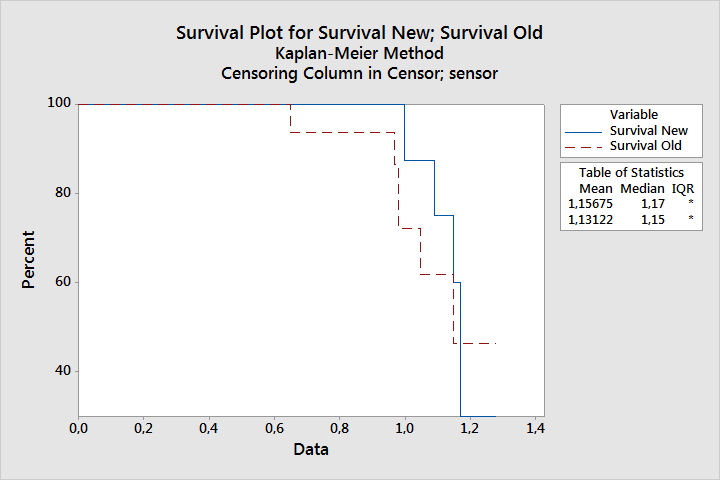
\includegraphics[scale=0.75]{Kaplan1.png}
\caption{A figure of the survival plot for new and old tires}
\label{Kaplan1}
\end{figure}
As we can see on the figure the median and the mean of the new tires are slightly higher than for the old tires. And by the log-Rank test done by minitab, we can conclude that the old tires are not as good as the new tires, if we use 95 \% confidence.

\section*{b)} 	% ok %%%%%%%%%%%%%%%%%%%%%%%%%%%%%%%%%%%%%%%%%%%%%%%%%%%

Regression Table



\begin{table}[h!]
\centering

\begin{tabular}{ l c c c c c r }

                   &          & Standard &          &    &  95,0\% & Normal CI\\
Predictor   &           Coef  &    Error &     Z    &  P &     Lower  &    Upper\\
Intercept   &       -5,18665  &  2,84774 & -1,82 & 0,069 &  -10,7681 &  0,394816\\
Tire age    &     -0,0560298  &0,0717152&  -0,78 & 0,435 & -0,196589 & 0,0845294\\
Wedge gauge     &   0,618075   &0,233062&   2,65 & 0,008 &  0,161282 &   1,07487\\
Interbelt gauge &   0,677893   &0,305756&   2,22 & 0,027 & 0,0786229 &   1,27716\\
EB2B            &   0,735087   &0,529309&   1,39 & 0,165 & -0,302340 &   1,77251\\
Peel force      &    1,97579   &0,780630&   2,53 & 0,011 &  0,445789 &   3,50580\\
Carbon black    &    2,79784   & 2,07499&   1,35 & 0,178 &  -1,26906 &   6,86475\\
W x P           &   -1,23881   &0,475896&  -2,60 & 0,009 &  -2,17155 & -0,306075\\
Shape           &    16,7698   & 4,32613&        &       &   10,1144 &   27,8044\\

\end{tabular}
\caption{Regression with Life Data, from minitab.}
   \label{model}
\end{table}


With Log-Likelihood $= 10,056$. We see that wedge gauge, Interbelt gauge, Peel force and W x p are significant covariants on a 5 \% level. The shape-parameter is bigger than one, suggesting that the failure rate increases over time, which seems reasonable when comparing to figure \ref{Kaplan1}.\\
The values in our table are quite different from the ones in the article, probably because of the difference in models. But some of the p-values and the $z$ and $t$ values in the different models are quite similar. Also the significant covariants are the same.

\section*{c)} 	% ok %%%%%%%%%%%%%%%%%%%%%%%%%%%%%%%%%%%%%%%%%%%%%%%%%%%

\begin{table}[h!]
\centering

\begin{tabular}{ l c c c c c r }

                   &          & Standard &          &    &  95,0\% & Normal CI\\
Predictor   &           Coef  &    Error &     Z    &  P &     Lower  &    Upper\\
Intercept   &     -1,35968  &0,316173 & -4,30&  0,000&  -1,97937 & -0,739994\\
Wedge gauge &     0,570659 & 0,184221 &  3,10&  0,002&  0,209593 &  0,931725\\
Interbelt gauge&  0,467936 & 0,144704 &  3,23&  0,001&  0,184322 &  0,751551\\
Peel force     &   1,62726 & 0,452442 &  3,60&  0,000&  0,740486 &   2,51403\\
W x P          &  -1,09370 & 0,292382 & -3,74&  0,000&  -1,66676 & -0,520641\\
Shape          &   16,7486 &  4,12438 &      &       &   10,3364 &   27,1387\\


\end{tabular}
\caption{Regression with Life Data with non-significant data taken out, from minitab.}
   \label{rep}
\end{table}
Log-Likelihood $= 6,621$.
Compared to table 3 in the article all values are quite different. Probably because of the difference in model.

\section*{d)}

\begin{table}[h!]
\centering

\begin{tabular}{ l c c c c c r }
& Lower quartile & median & Upper quartile & $1.0$ & $1.2$&$1.5$\\
Bad tire& 0.84 & 1.12 & 1.50 & 0.83 & 0.24 & 0,00\\
Good tire & 1.12 & 2.63 & 6,20 & 0.99 & 0.99 & 0.99\\

\end{tabular}
\caption{Table with interesting values for good and bad tires.}
   \label{expe}
\end{table}
So clearly a "good tire" lasts longer than a "bad tire".

\section*{e)}
We now want to compare the model in section b) with the model in section c) and the Weibull model using no covariants. For this we want compare the log-likelihood values.

$H_0:$ models are the same versus $H_1: $ the models are different.

Comparing the models in b) and c) yields

$\chi^2_4=9.49$ on a significant level of $\alpha = 0.05$. Twice difference in log-likelihood is $2(10.056-6.621) =6.87 $.
$P(\chi^2_5 > 6.87) = 0.15 $ And we therefore do not reject $H_0$. And conclude that the reduced model from c) is sufficient when estimating the lifetime of the tires.  \\


In the model with no covariants minitab gives log-likelihood $= -4.958$. $2(10.056-(-4.958)) =30.028 $, $P(\chi^2 > 30.028) < 0.001$. We therefore reject the hypothesis that the model without covariants, and the model with all covariants are equal. 

\section*{f)} % ok

The Cox-model gives the following expression $$ z_0(t;x) =z_0(t) e^{\beta_1x_1+\beta_2x_2+\beta_3x_3+\beta_4x_4} $$ The main difference between the cox model from the reduced model and the full model is the number of $\beta$-s. But the models should give the same probability for the same time. 
The hazard-rate for the Weibull-regression is $$ z_0(t) = z_0(t) e^{-\alpha(\beta_1x_1+\beta_2*x_2+\beta_3 x_3+\beta_4 x_4)} $$

So we see that the difference is the "$-\alpha$" term. Which only means that the $\beta$ in one is the same as $-\alpha \beta$ in the other.  The estimates for $ \beta $-s in the Weibull regression model is given in table \ref{model} and \ref{rep}, for the full, and reduced model.

\section*{g)}

\begin{figure}
         \centering
         \begin{subfigure}[b]{0.4\textwidth}
                 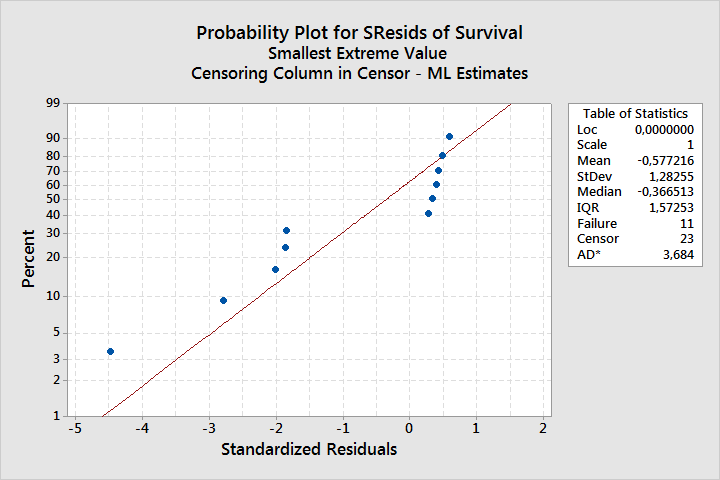
\includegraphics[width=\textwidth]{stdful}
                 \caption{Residual standard plot of the full model}
                 \label{stdful}
         \end{subfigure}
         \begin{subfigure}[b]{0.4\textwidth}
                 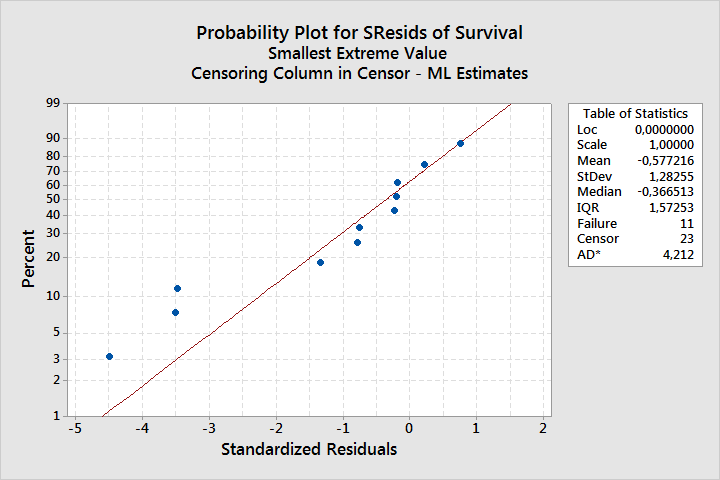
\includegraphics[width=\textwidth]{stdred}
                 \caption{Residual standard plot of the reduced model}
                 \label{stdred}
         \end{subfigure}
         \\
         \begin{subfigure}[b]{0.4\textwidth}
                 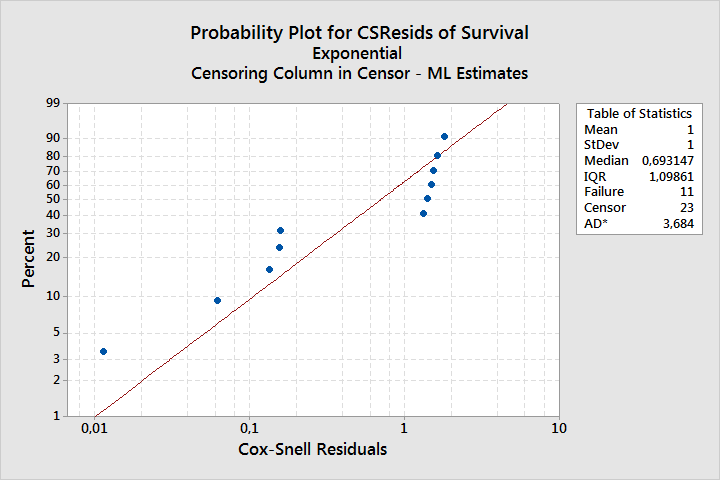
\includegraphics[width=\textwidth]{coxful}
                 \caption{Residual Cox-Snell plot of the full model}
                 \label{coxful}
         \end{subfigure}
         \begin{subfigure}[b]{0.4\textwidth}
                 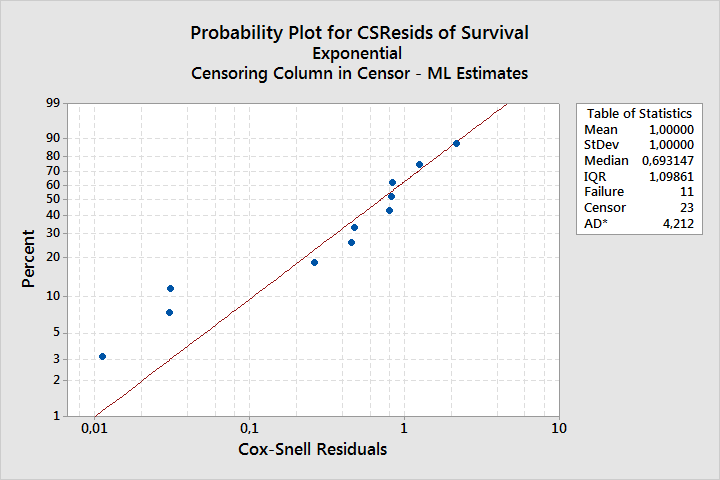
\includegraphics[width=\textwidth]{coxred}
                 \caption{Residual Cox-Snell plot of the reduced model}
                 \label{coxred}
         \end{subfigure}
         \caption{Plots of reciduals}\label{4x}
\end{figure}
When deriving the Cox-Snell residuals, we start by taking the logarithm of the survival function to the model we use, which is weibull in this case.
$$ \ln T_i = \beta _0 +  \sum \limits_{k = 1}^{n} \beta_k x_k+\sigma U_i   $$
$$ R_{T_i} =  1- \phi ( \frac{\ln t-\beta _0 -  \sum \limits_{k = 1}^{n} \beta_k x_k}{\sigma}) $$
$$ V_i = -\ln R_{T_i}(T_i) = -\ln[ 1- \phi ( \frac{\ln t-\beta _0 -  \sum \limits_{k = 1}^{n} \beta_k x_k}{\sigma}) ] $$
For the Weibull -distribution we have $$ \ln T = \beta_0 + \sum \limits_{i=1}^k+\frac{1}{\alpha} W $$ which is the same as for the cox-model, and the of course gives the same residuals. This explains why the residual plots are the same for the two models. I also think the reduced model gives a better fit for the model.



\begin{figure}
         \centering
         \begin{subfigure}[b]{0.5\textwidth}
                 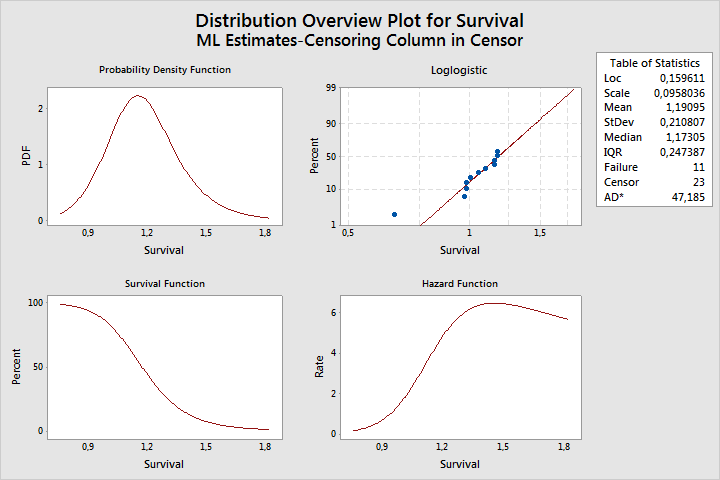
\includegraphics[width=\textwidth]{loglog}
                 \caption{loglogistics plot over interesting data}
                 \label{loglog}
         \end{subfigure}
         \begin{subfigure}[b]{0.5\textwidth}
                 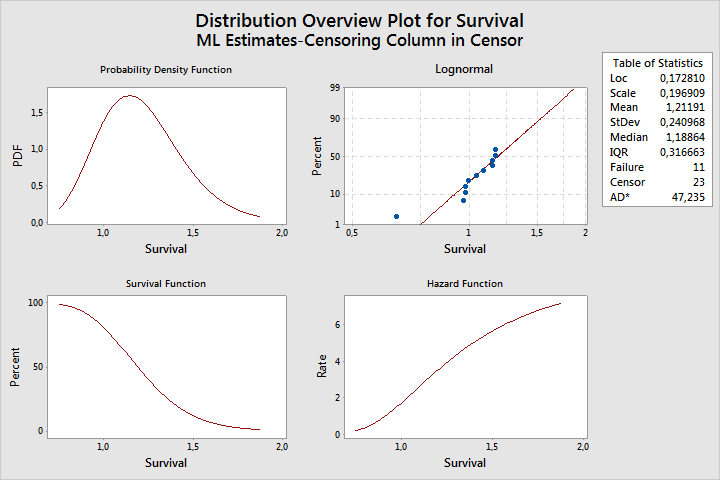
\includegraphics[width=\textwidth]{lognorm}
                 \caption{LogNormal plot over interesting data}
                 \label{lognorm}
         \end{subfigure}

         \caption{Plots of different fitted modells.}\label{2x}
\end{figure}
When comparing all the plots from plot \ref{4x} and plot \ref{2x}, I would say the reduced cox-snell/weibull gives the best estimate. Loglogistics and lognormal gives a distinct "s"-shape, which means that the model is probably wrong.

\section*{h)}

\begin{figure}[h!]
\centering
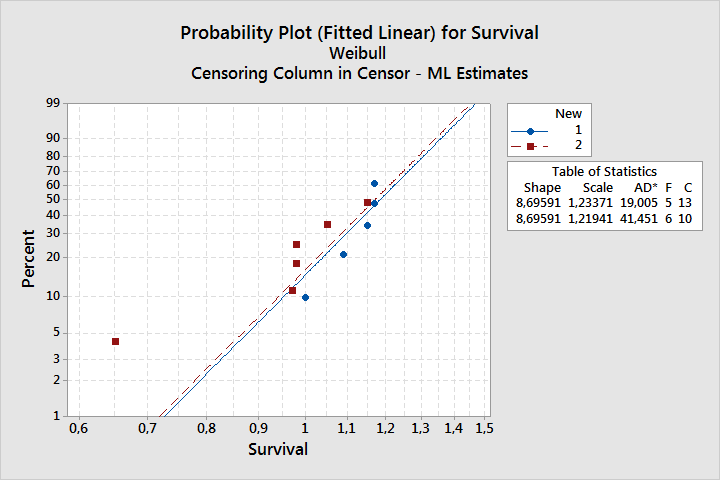
\includegraphics[scale=0.75]{siste.png}
\caption{Probability plot for accelerated lifetime testing}
\label{siste}
\end{figure}
From plot \ref{siste} we can see that the reduced model gives a better approximation for the regression than the full model, since it is closer to the line. We also have one point way of in the full model.


\end{document}